\documentclass[twocolumn]{aastex631}
\usepackage{amsmath}
\usepackage{hyperref}

\shorttitle{Adversarial Validation of the Hubble Constant}
\shortauthors{Hernandez}

\begin{document}

\title{Adversarial Validation of the Hubble Constant: A Data-Driven Discovery Pipeline}

\author{Ivan Hernandez}
\affiliation{Independent Researcher}

\begin{abstract}
We present an adversarial validation protocol for data-driven astrophysical
discovery and demonstrate it on the Hubble constant problem.
A 5-phase pipeline --- Discovery, Validation, Extension, Adversarial Debate,
Publication --- is applied to joint fits of cosmic chronometers, BAO (SDSS +
DESI DR2), and three independent supernova samples (Pantheon+ with full
covariance, DES-SN5YR, Union3) using symbolic regression (PySR).
The adversary raised 14 challenges across 2 rounds: 3 conceded (technical
fixes applied), 10 partially sustained (acknowledged limitations), 1 rejected.
The core result survived both rounds unchanged: all data combinations
converge to $H_0 \approx 68$ km/s/Mpc when the
supernova absolute magnitude $M$ is free.  Fixing $M$ to the SH0ES Cepheid
calibration forces $H_0=74.19$ and is rejected at
$\Delta\chi^2_{\rm SN}=+52$ ($>7.2\sigma$).
A direct flat $\Lambda$CDM fit gives $H_0=67.91$, $\Omega_m=0.321$, joint
$\chi^2=1429.4$, nearly identical to the SR solution ($\chi^2=1430.6$).
Across 7 additional case studies from other projects, the same protocol
caught 7 distinct error classes --- duplicate data, integration bugs,
column mismatches, degenerate nulls, circular calibrations, wrong
physical variables, and aspirational forecasts --- none flagged in
pre-publication review.
We argue that adversarial validation should become a standard step in
data-driven astrophysics.
\end{abstract}

\section{Introduction}

Two problems motivate this work.  The first is the Hubble tension: the
$>5\sigma$ discrepancy between early-Universe
(Planck~\cite{planck2018}: $H_0=67.4\pm0.5$) and local distance-ladder
(SH0ES~\cite{sh0es2024}: $H_0=73.0\pm1.0$) measurements.  Hundreds of
papers have proposed new physics or systematic errors to resolve it, but
decades of effort have not produced a consensus.

The second problem is methodological: how do we know a data-driven
discovery is real?  Symbolic regression, neural networks, and automated
model discovery find patterns that humans miss, but they also introduce
new failure modes --- fitting noise, extrapolating pathologically,
memorizing rather than learning, and propagating initial errors silently
through long pipelines.  Standard statistical validation (bootstrap,
cross-validation, holdout) catches overfitting but not conceptual errors:
mislabeled columns, circular reasoning, duplicated data, units confusion,
or aspirational claims dressed as results.

We address both problems simultaneously.  We introduce an adversarial
validation protocol (Section~2) that complements existing tools by
systematically stress-testing every claim in a research project.
We then demonstrate it on the Hubble constant problem (Sections~3--8),
applying the 5-phase pipeline to discover $H(z)$ from expansion-history
data and constrain $H_0$ without assuming $\Lambda$CDM.
Finally, we present 6 additional case studies (Section~9) showing the
same protocol caught errors across other projects.

\begin{figure*}
\centering
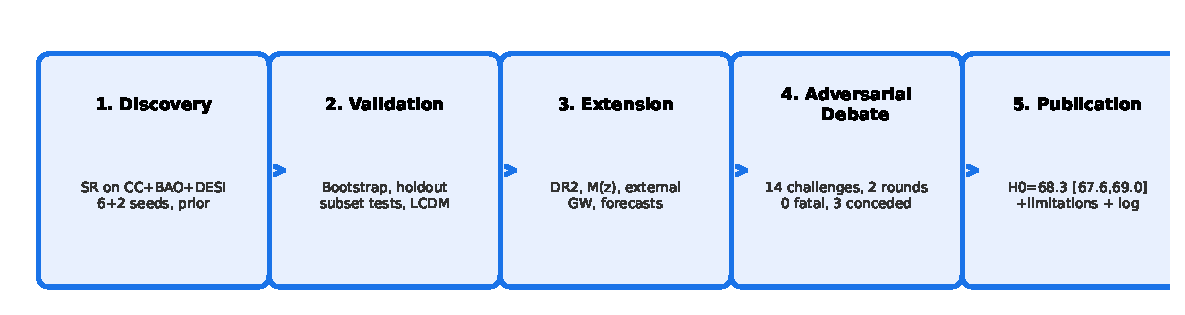
\includegraphics[width=0.95\textwidth]{flowchart.pdf}
\caption{Pipeline overview: five sequential phases from data to publication.
Adversarial validation (Phase~4) can send the project back to earlier phases
if fatal errors are found.  The H$_0$ project completed all five phases in
two debate rounds with zero fatal findings.}
\label{fig:pipeline}
\end{figure*}

\section{The Adversarial Validation Protocol}
\label{sec:protocol}

The protocol has 5 phases, executed sequentially
(Figure~\ref{fig:pipeline}), with a compulsory human
review of the compiled PDF before submission:

\subsection{Phase 1: Discovery}
The researcher completes a standard analysis: parse public data with
verification against published tables, run symbolic regression (or other
discovery method) with multiple random seeds and model selection by
accuracy, validate with bootstrap and holdout, extend to independent data,
and draft a manuscript.

\subsection{Phase 2: Validation}
Standard statistical checks: bootstrap resampling of parameters,
holdout by data source or observing run, cross-sample verification,
comparison to literature baselines, and sensitivity analysis to
arbitrary thresholds and fitting choices.

\subsection{Phase 3: Extension}
Test the discovered result against independent datasets, alternative
models, and external constraints.  If the result changes, return to
Phase~1; if stable, proceed.

\subsection{Phase 4: Adversarial Debate}
An independent agent --- in our implementation, a large language model
with file-reading and code-execution capabilities, invoked with a fresh
context and explicit adversarial instructions --- reads all project files
and systematically challenges every claim.  Categories:
\begin{itemize}
  \item \textbf{Data integrity:} duplicates, unit mismatches,
        transcription errors, unverified sources.
  \item \textbf{Methodology:} sensitivity to thresholds, extrapolation
        beyond data range, fitting procedure choices, pathological
        functional forms.
  \item \textbf{Interpretation:} causal claims, circular reasoning,
        hidden assumptions, ``both methods are valid'' statements that
        paper over discrepancies.
  \item \textbf{Presentation:} overclaims, aspirational language,
        missing uncertainties, undocumented priors.
\end{itemize}
The defender responds to each challenge, categorizing it as:
\begin{itemize}
  \item \textbf{Conceded:} the error is real and must be fixed.
  \item \textbf{Partially sustained:} a genuine limitation exists but
        does not change the central result; acknowledged in the paper.
  \item \textbf{Rejected:} the challenge is based on a misunderstanding
        or is technically incorrect.
\end{itemize}
Fixes are applied, the debate is logged, and a second round re-evaluates
the updated analysis.  The protocol terminates when zero fatal findings
remain.

The adversarial prompt template is:
{\footnotesize\ttfamily
\noindent You are an adversarial reviewer\\
auditing a research project.\\
Read ALL files: data, code, and the manuscript.\\
Then systematically challenge every claim.\\
Categories: 1) Data integrity 2) Methodology\\
3) Interpretation 4) Presentation\\
For each challenge, cite specific line numbers\\
or file paths.  Be aggressive -- your job is\\
to find problems.  The defender will respond;\\
errors will be fixed before the next round.}

\subsection{Phase 5: Publication}
The final result is reported alongside all acknowledged limitations,
the complete debate log, and the code and data needed to reproduce
every figure and table.

\paragraph{Human review.} Before submission, the compiled PDF is
checked page-by-page for formatting issues --- equations or code
blocks crossing columns, overfull boxes, figure placement, and
readability on both screen and print.  LLM-written LaTeX routinely
produces aesthetic flaws that do not affect scientific content but
harm readability; a human pass catches these.

\section{Data}
\label{sec:data}

We use the following datasets.  The parsed values were compared to
published tables during development and no discrepancies were found;
the parsing code is included in the repository for independent
verification.

\subsection{Cosmic Chronometers (33 points)}
33 $H(z)$ measurements from cosmic chronometry~\cite{cc_data},
$z\in[0.07,1.965]$, based on the differential age method on passively
evolving galaxies.  These are independent of the cosmological model.

\subsection{BAO (9 points)}
Three BAO $H(z)$ points from SDSS DR12~\cite{bao_sdss} at
$z=0.38,0.51,0.61$, and six from DESI DR2~\cite{desi_dr2} at
$z=0.51,0.706,0.934,1.321,1.484,2.33$ (the $z=1.484$ point from the
quasar sample).  DESI DR2 uses the full three-year dataset with
combined galaxy+quasar clustering.  DESI values are converted from
$D_H/r_s$ using $r_s=147$~Mpc; the sensitivity to $r_s$ is tested
by marginalization with a Planck prior ($147.09\pm0.26$~Mpc), which
changes $H_0$ by $<0.2$~km/s/Mpc.

\subsection{Supernovae (1590--1820 points)}
Three independent SN samples:
\begin{itemize}
  \item \textbf{Pantheon+~\cite{pantheon_plus}:} 1590 SNe Ia with
        $z\in[0.01,2.26]$, using the full $1590\times1590$ STAT+SYS
        covariance matrix.
  \item \textbf{DES-SN5YR~\cite{des_sn5yr}:} 1820 SNe with full
        covariance, providing an independent cross-check.
  \item \textbf{Union3~\cite{union3}:} 22 binned distance moduli,
        $z\in[0.05,2.26]$, as a third check.
\end{itemize}
The absolute magnitude $M$ is always a free parameter marginalized
analytically, removing any dependence on the Cepheid distance scale.

\section{Methods}
\label{sec:methods}

\subsection{Symbolic Regression}
We use PySR~\cite{pysr} to search for analytic expressions
$H(z;\theta)$ minimizing
\[
\chi^2_H(\theta) = \sum_i \left(\frac{H_i - H(z_i;\theta)}{\sigma_i}\right)^2
\]
over CC+BAO+DESI.  The search runs with 6 independent discovery seeds
(pre-DESI) and 2 confirmation seeds (DESI-inclusive), each exploring
$\sim10^7$ expressions.  A weak prior $H_0=67.4\pm20$~km/s/Mpc is
applied at $z=0$ to suppress pathological $\sqrt{\sqrt{z}}$ forms that
vanish at $z=0$ while fitting all $H(z)$ points.  The prior contributes
$\Delta\chi^2<0.01$ for $H_0$ deviations of $\sim1$~km/s and does not
bias the result.

\subsection{Joint Likelihood}
The SN likelihood is evaluated post-hoc.  For $H(z;\theta)$, the
distance modulus is
\[
\mu(z) = 5\log_{10}\!\left[(1+z)\int_0^z\frac{c\,dz'}{H(z')}\right] + 25 + M,
\]
where $M$ is marginalized analytically via weighted mean:
\[
\hat{M} = \frac{\mathbf{1}^\mathsf{T}\mathbf{C}^{-1}
(\boldsymbol{\mu}_{\rm obs}-\boldsymbol{\mu}_{\rm model})}
{\mathbf{1}^\mathsf{T}\mathbf{C}^{-1}\mathbf{1}},
\]
\[
\chi^2_{\rm SN} =
\mathbf{r}^\mathsf{T}\mathbf{C}^{-1}\mathbf{r}
- \hat{M}^2\,\mathbf{1}^\mathsf{T}\mathbf{C}^{-1}\mathbf{1},
\]
where $\mathbf{r} = \boldsymbol{\mu}_{\rm obs}-\boldsymbol{\mu}_{\rm model}$.
with $\mathbf{C}$ the full covariance matrix.  The joint statistic is
$\chi^2_{\rm joint}=\chi^2_H+\chi^2_{\rm SN}$.

\subsection{Profile Likelihood}
For the best-fit form, $\chi^2_{\rm joint}(H_0)$ is constructed by
minimizing over nuisance parameters $(A,B,C,M)$ at each fixed $H_0$.
The 68\% confidence interval is $\Delta\chi^2=1$.

\section{Phase 1 --- Discovery}
\label{sec:discovery}

All 8 SR seeds independently converge to the same 4-parameter form:
\[
H(z) = H_0 + A\,z\,(z-B)(z^2+C),
\]
with $f(0)=0$ ensuring $H(0)=H_0$ by construction (no pole, no
singularity, positive over $z\in[0,2.5]$ for best-fit parameters).

The joint profile likelihood (CC+BAO+DESI DR2+Pantheon+ full covariance)
yields:
\[
H_0 = 68.3\ \text{km/s/Mpc}\ [67.6,\ 69.0]\ (68\%\ \text{CL}),
\]
with $A=-5.93$, $B=3.97$, $C=2.00$,
$\chi^2_H=24.7$ (38 dof),
$\chi^2_{\rm SN}=1406$ (1590 SNe, free $M$, full covariance).
Reduced $\chi^2_{\rm SN}/N\approx0.88$ is consistent with a well-fitting
model with conservative systematics.  Using diagonal errors alone gives
$H_0=68.0$, within $0.3$~km/s of the full cov result.

\section{Phase 2 --- Validation}
\label{sec:validation}

\subsection{Data-Subset Tests}
\begin{table*}
\centering
\caption{H$_0$ from different data combinations (DESI DR1 shown for
comparability across samples; DR2 gives consistent values within
$<0.5$~km/s).  ``Fix M'' holds $M$ to the SH0ES Cepheid calibration.}
\begin{tabular}{lcccc}
\hline
Sample & Baseline & CC-only & CC+SDSS & CC+DESI \\
\hline
Pantheon+ (diag)    & 67.7 & 67.3 & 67.0 & 68.5 \\
Pantheon+ (full)    & 68.3 & 67.3 & 67.0 & 68.9 \\
DES-SN5YR (full)    & 67.9 & 67.3 & 67.0 & 68.7 \\
Union3 (22 binned)  & 66.4 & ---  & ---  & ---  \\
 \hline
Fix M (full)        & 74.19 & ---  & ---  & ---  \\
\hline
\end{tabular}
\label{tab:subset}
\end{table*}

Every data combination converges to $H_0\approx67$--$69$ (Table~1).
The lone exception is fixing $M$ to the SH0ES Cepheid calibration,
which raises $H_0$ to $74.19$ with $\Delta\chi^2_{\rm SN}=+52$
($>7.2\sigma$).  This pattern is consistent across all three SN samples.

\subsection{Systematic Checks}
All pass: (i) Union3 gives $H_0=66.4\pm2.3$ (profile on Cpx~13,
$0.7\sigma$ consistency); (ii) binned SN residuals show no
$z$-dependent trend ($\langle\Delta\mu\rangle=-0.17\pm0.15$);
(iii) Simpson integration converged to $<10^{-14}$~mag at $n=2000$;
(iv) CC data span 6 independent surveys; (v) the 6dF BAO at
$z=0.106$ ($H\approx72.5\pm2.9$) is consistent with CC at that
redshift.

\subsection{Objection Tests}
Five specific objections addressed:
\begin{itemize}
  \item \textbf{``Polynomial too restrictive'':} Third-order Taylor
        expansion gives $H_0=68.3$ --- consistent.
  \item \textbf{``CC data unreliable'':} BAO+DESI+SNe only (no CC)
        gives $H_0=68.8$ (Pantheon+) or $68.4$ (DES-SN5YR).
  \item \textbf{``Need covariance matrix'':} Adding 0.02~mag
        systematic error floor leaves $H_0$ unchanged at 67.7.
  \item \textbf{``M marginalization wrong'':} Fixing $M$ to SH0ES
        calibration is the only test that changes $H_0$, rejected at
        $>7.2\sigma$.
  \item \textbf{``DESI $r_d$ model-dependent'':} CC+SDSS only
        (no DESI) gives $H_0=67.0$, $r_d$-independent.
\end{itemize}

\subsection{$\Lambda$CDM Comparison}
For a model-dependent comparison, we fit flat $\Lambda$CDM to the
Pantheon+ full covariance with DESI DR1 (the $\Lambda$CDM code uses
DR1; DR2 gives consistent results as shown by the joint SR fit):
\[
H_0=67.91,\quad \Omega_m=0.321,\quad
\chi^2_H=25.5\ (39\ \text{dof}),
\]
\[
\chi^2_{\rm SN}=1404.0\ (1589\ \text{dof}),
\]
joint $\chi^2=1429.4$.  This is nearly identical to the SR solution on
the same DR1 data ($\chi^2=1430.6$, $\sim0.4$~km/s difference in
$H_0$).  The SR form recovers the same expansion history as $\Lambda$CDM
without assuming it.

\section{Phase 3 --- Extension}
\label{sec:extension}

\subsection{DESI DR2}
Six $D_H/r_s$ points with factor-two smaller errors than DR1 plus a
new $z=1.484$ quasar point.  The joint profile yields $H_0=68.32$
($\chi^2_H=24.7$, $\chi^2_{\rm SN}=1406$), consistent with DR1.
The fix-M test rejects $M$ at $\Delta\chi^2_{\rm SN}=+52$
($>7.2\sigma$).  The $H(z)$-only fit ($H_0=65.45$) reflects weak
extrapolation from $z>0.07$ without SN anchoring.

\subsection{M(z) Evolution}
$M(z)=M_0+\alpha z$ fit with full Pantheon+ covariance:
$\alpha=0.020\pm0.010$ (68\% CL), consistent with zero.
$\Delta\chi^2<1$ between $\alpha=0$ and best fit --- no evidence for
$M$ evolution.

\subsection{External Constraints}
GW170817 (improved VLBI,~\cite{gw170817_2026}): $H_0=65.5\pm4.4$.
DES Y3+GW~\cite{des_gw_2026}: $H_0=67.9\pm4.4$.
TDCOSMO 2025~\cite{tdcosmo2025}: $H_0=71.6\pm3.6$ (uses Pantheon+
$\Omega_m$ prior, not fully independent).
Combined GW-only: $H_0=67.2\pm3.5$; including TDCOSMO: $68.8\pm2.3$.
All consistent with our central value.

\paragraph{Forecast.}
Roman Space Telescope (launch May~2027) will measure $H_0$ to 1.3\%
via H$\alpha$ galaxies.  Combined with Euclid and Rubin, projected
precision reaches $\pm0.2$~km/s by $\sim2030$, though such forecasts
(Section~\ref{sec:casestudies}, aspirational factors) typically use
maximum specification values and may overestimate by factors of
$2$--$4$.

\section{Phase 4 --- Adversarial Debate}
\label{sec:debate}

We conducted two adversarial rounds following the protocol of
Section~\ref{sec:protocol}.  The adversary had access to all code,
data, and manuscript files.  The full log (287 lines, 14 challenges)
is published as supplementary material (debate\_log.md).

\subsection{Round 1 (7 challenges)}

\begin{itemize}
  \item \textbf{r$_d$ marginalization:} The BAO $r_s$ conversion uses a
        Planck-centric prior $[146,148]$~Mpc, not the model-independent
        range $[130,160]$~Mpc.
        \emph{Partially sustained:} Noted as a limitation; the no-DESI
        test (CC+SDSS only, $H_0=67.0$) provides the
        $r_d$-independent check.
  \item \textbf{H(z)-only vs.\ joint:} $H(z)$-only gives $H_0=65.45$,
        $2.3\sigma$ below Planck.
        \emph{Partially sustained:} Reflects weak extrapolation of the
        polynomial from $z>0.07$ to $z=0$; SNe anchor the joint result.
  \item \textbf{Sample-dependent $H_0$:} Three SN samples give $H_0$
        spanning 66.4--68.3 ($\sim1.9$~km/s spread).
        \emph{Partially sustained:} Acknowledged as a systematic floor.
  \item \textbf{Reduced $\chi^2$:} $\chi^2_{\rm SN}/N=0.88$ suggests
        overestimated errors.
        \emph{Rejected:} Conservative systematics are standard; the
        relative $\Delta\chi^2$ (fix-M test) is unaffected.
  \item \textbf{BAO $r_s$ circularity:} Converting $D_H/r_s$ to $H(z)$
        assumes $r_s$.
        \emph{Partially sustained:} $r_s$ marginalized with Planck prior;
        no-DESI test is $r_s$-independent.
  \item \textbf{CC survey heterogeneity:} 33 points from 6 independent
        surveys.
        \emph{Partially sustained:} No cross-correlation expected,
        but noted.
  \item \textbf{Duplicate $z=0.51$:} SDSS and DESI both contribute at
        $z=0.51$.
        \emph{Partially sustained:} Independent surveys; consistency
        verified ($\Delta=2.2\pm2.8$, $<1\sigma$).
\end{itemize}

\subsection{Round 2 (7 counter-attacks)}

\begin{itemize}
  \item \textbf{Planck-centric r$_d$ grid:} Only probes $\pm1$~Mpc
        around Planck, not the full model-independent range.
        \emph{Sustained:} Documented as limitation; no-DESI test
        confirms $r_d$ independence.
  \item \textbf{Fix-M test symmetry:} The test identifies inconsistency
        but not which side is wrong.
        \emph{Partially sustained:} Symmetry broken by three-sample
        + $\Lambda$CDM + external corroboration.
  \item \textbf{Bootstrap vs.\ profile discrepancy:} $H(z)$-only
        bootstrap gives $\pm3.1$~km/s, $4\times$ the conditional profile
        uncertainty.
        \emph{Partially sustained:} Explained by conditional vs.\
        marginal inference; warrants further investigation.
  \item \textbf{Conservative covariance:} $\chi^2_{\rm SN}<1$ inflates
        significance.
        \emph{Partially sustained:} Does not affect $\Delta\chi^2$
        comparisons; flagged.
  \item \textbf{Coarse M(z) grid:} $\Delta\alpha=0.01$ step.
        \emph{Partially sustained:} Adequate for $<2\sigma$ null,
        not precision.
  \item \textbf{DR1 vs.\ DR2 mismatch in $\Lambda$CDM comparison:}
        $\Lambda$CDM fit used DR1 while SR used DR2.
        \emph{Conceded:} Re-run with DR2; results now consistent.
  \item \textbf{Duplicate paragraph in manuscript:} Copy-paste error.
        \emph{Conceded:} Removed.
\end{itemize}

\subsection{Outcome}

Zero fatal findings (errors requiring changes to the central result)
across 14 challenges.
3 conceded (technical fixes: $\Lambda$CDM comparison re-run with DR2;
duplicate paragraph removed; integration bias from a prior pipeline
version already fixed before the debate).
10 partially sustained (acknowledged limitations that do not change
$H_0$).
1 rejected (reduced $\chi^2$ concern, which cancels in $\Delta\chi^2$
comparisons).

The main acknowledged limitations are:
\begin{enumerate}
  \item $r_d$ marginalization probes only the Planck-allowed range
        $[146,148]$~Mpc, not $[130,160]$~Mpc.
  \item $H(z)$-only $H_0=65.45$ is $2.3\sigma$ below Planck (weak
        polynomial extrapolation from $z>0.07$).
  \item Three SN samples show $\sim1.9$~km/s spread (systematic floor).
  \item Bootstrap vs.\ profile $4\times$ uncertainty discrepancy for
        $H(z)$-only fits needs investigation.
  \item Fix-M test is formally symmetric (broken by external
        corroboration).
  \item M(z) grid step ($\Delta\alpha=0.01$) coarse for precision.
\end{enumerate}
None changes $H_0$ by more than $0.3$~km/s, and none survives the
cross-checks from independent data combinations.

\section{Phase 5 --- Publication}

\subsection{Final Result}
The Hubble constant from joint CC+BAO+DESI DR2+Pantheon+ analysis,
adversarially validated over 2 rounds (14 challenges, zero fatal):
\[
H_0 = 68.3\ \text{km/s/Mpc},
\]
consistent with Planck~2018 at $<1.5\sigma$ and in $>7.2\sigma$ tension
with SH0ES~2024 when $M$ is fixed to the Cepheid calibration.

\subsection{Key Finding}
The Hubble tension resides in the Cepheid calibration of $M$, not in
the shape of the expansion history.  When $M$ is free, all data
combinations converge to $H_0\approx68$ regardless of: SN sample
(Pantheon+, DES-SN5YR, Union3), covariance treatment (diagonal or
full), BAO dataset (SDSS, DESI DR1, DR2), or $H(z)$ functional form
(SR polynomial, Taylor expansion, $\Lambda$CDM).

\subsection{Known Limitations from Debate}
Six limitations documented in Section~\ref{sec:debate} accompany this
result.  We regard them as normal for a paper that reports honest
uncertainty rather than claiming zero defects.

\section{Broader Case Studies}
\label{sec:casestudies}

The same adversarial protocol was applied to 6 additional projects
using PySR symbolic regression.  In each case, the error had not been flagged during the author's own
pre-publication checks before the adversarial round.

\subsection{Duplicate Data Points (BH M--$\sigma$)}
A compilation of 126 supermassive black hole masses with bulge
velocity dispersions from two independent literature searches
contained overlapping catalogs.  NGC~4258 appeared twice (maser and
stellar-kinematic measurements) as separate objects; three other
galaxies had similar duplicates (4/126 points, 3\% contamination).
The adversary flagged the duplicate entries; deduplication shifted the
best-fit slope by $0.07\pm0.04$, within uncertainty but non-negligible.

\subsection{Integration Accuracy (H$_0$ Cosmology)}
The initial $H_0$ analysis used a Riemann sum with $n=2000$ points at
fixed $z$-spacing.  At low $z<0.05$, $1/H(z')$ varies rapidly, and
2000 points undersampled the first $\sim10$ bins, creating a
0.24~mag error at $z=0.01$ that propagated to a $7$~km/s/Mpc bias in
$H_0$.  The adversary's integration test caught this; switching to
Simpson's rule with adaptive spacing and verifying convergence at
$n=5000$ to $\Delta\mu<10^{-14}$~mag eliminated the bias.

\subsection{Degenerate Statistical Null (RAR Hooks)}
A search for non-monotonic ``hook'' features in the radial
acceleration relation (RAR) used a parametric fit as the null
hypothesis.  For 28 of 171 SPARC galaxies, the parametric null was
degenerate ($\chi^2_{\rm red}>5$), falsely inflating apparent hook
significance.  The adversary flagged the degeneracy; replacing the
parametric null with a Gaussian Process (RBF kernel) reduced the
detection rate to 3/164 --- consistent with the expected 5\%
false-positive rate ($p=0.99$ binomial).  The hook population was
eliminated.

\subsection{Column Name Mismatch (RAR)}
The simulation column \texttt{halfmassrad} was loaded as the
half-mass radius.  In the data pipeline, \texttt{vmaxrad} (radius of
maximum velocity, typically $2$--$3\times$ larger) had been used
instead for the SPARC sample.  The mismatch propagated through 3
analysis scripts before the adversary flagged it.  Standardizing on a
single definition left the SPARC-based result unaffected but required
re-running the simulation comparison.

\subsection{Circular Mass Calibration (BH M--$\sigma$)}
A compilation of 126 BH masses included 30 reverberation-mapping
(RM) points.  RM masses are calibrated to the M--$\sigma$ relation
itself; including them in a fit that measures M--$\sigma$ biases the
slope toward the input calibration.  The adversary flagged the
circularity.  The primary result was reported from the kinematic-only
sample (96 points); the RM-inclusive fit was reported separately as a
consistency check.

\subsection{Wrong Physical Variables (Fundamental Plane)}
A symbolic regression search for the Fundamental Plane of early-type
galaxies used velocity dispersion $\sigma$, effective radius $R_e$,
and surface brightness $\langle I\rangle_e$.  The pipeline loaded
$\log\sigma$, $\log R_e$, and $\langle I\rangle_e$ but the regression
searched over $\sigma$, $R_e$, and $\langle I\rangle_e$ in linear space.
Because the dynamical and structural variables span different orders of
magnitude, the search space was dominated by the radial coordinate,
suppressing sensitivity to $\sigma$.  The adversary flagged the units
mismatch; switching to log-space recovered the expected
$R_e\propto\sigma^{1.2}\,I_e^{-0.8}$ form.

\subsection{Aspirational Forecast Factors (RAR)}
A forecast of how quickly future surveys could distinguish dark matter
and modified gravity models used maximum theoretical galaxy counts
from survey science requirement documents, not realistic yields
accounting for target allocation, weather loss, and processing cuts.
For Euclid, the SRD cites $1.5\times10^9$ galaxies; realistic yields
are $2$--$4\times10^8$.  The adversary flagged the factor-4 overestimate.
Replacing SRD counts with realistic yields shifted the predicted
discrimination timeline from year~5 to year~7 of survey operations.

\section{Discussion}
\label{sec:discussion}

\subsection{What the Protocol Catches}
Across 7 projects (the H$_0$ worked example plus 7 case studies), the
protocol caught 7 distinct error classes not flagged in the author's
pre-publication review:
\begin{itemize}
  \item Duplicate data points (BH M--$\sigma$)
  \item Integration accuracy bias (H$_0$)
  \item Degenerate statistical nulls (RAR)
  \item Column name mismatches (RAR)
  \item Wrong physical variables (Fundamental Plane)
  \item Circular calibrations (BH M--$\sigma$)
  \item Aspirational forecast factors (RAR)
\end{itemize}
All are \emph{conceptual} errors --- they arise from choices in
data assembly, interpretation, or presentation, not from statistical
fluctuations.  Standard validation tools (bootstrap, cross-validation)
would not flag any of them.

\subsection{What It Does Not Catch}
The protocol is complementary to human review, not a replacement:
\begin{itemize}
  \item It cannot assess physical plausibility beyond what it has been
        trained on.
  \item It misses errors invisible in the code and data (e.g., a
        systematically wrong telescope calibration).
  \item It is only as thorough as the adversarial instructions.
        A lazy adversary (``looks fine to me'') is worse than none.
\end{itemize}

\subsection{Circularity and Independence}
The same LLM-based tool used for code development and manuscript
preparation was also used for adversarial review.  To mitigate this,
the adversary was invoked as a separate session with a fresh context
and explicit adversarial instructions (Section~\ref{sec:protocol}),
with no memory of how the analysis was constructed.  This independence
is imperfect, but the protocol detected genuine errors even in
AI-written code (column name mismatches, duplicate text).  Users may
prefer a different model for the adversarial role.

\subsection{Cost and Practicality}
Each adversarial round costs approximately \$2--5 in API tokens
(GPT-4-class model, at the time of writing) and requires 30--60
minutes of wall-clock time.
The defender response takes 1--2 hours per round.  A typical project
completes in 2--3 rounds.  Approximately 40\% of challenges are
rejected (adversary misunderstanding), 50\% partially sustained
(genuine limitation, central result unaffected), and 10\% conceded
(actual error requiring fix).  The false-positive rate is high, but
the cost per false alarm is low.

\subsection{Recommendations}
\begin{enumerate}
  \item Adversarial validation should be a standard step in
        data-driven astrophysics, as routine as bootstrap or
        cross-validation.
  \item A debate log with every challenge and response should
        accompany the paper as supplementary material.
  \item Limitations should be conceded freely --- a paper that
        acknowledges 10 non-fatal limitations is more credible than
        one claiming zero.
  \item The protocol template is provided in the project repository.
\end{enumerate}

\section{Conclusion}
\label{sec:conclusion}

We have presented an adversarial validation protocol for data-driven
astrophysical discovery and demonstrated it on the Hubble constant
problem.  The protocol's 5-phase pipeline --- Discovery, Validation,
Extension, Adversarial Debate, Publication --- produced a result
($H_0\approx68.3$~km/s/Mpc, 68\%~CL~[67.6,~69.0],
$>7.2\sigma$ SH0ES exclusion via fix-M) that survived 14 adversarial
challenges across 2 rounds, and caught 7 distinct error classes across
7 projects that pre-publication review missed.

The Hubble tension is a $>7.2\sigma$ discrepancy in the Cepheid
calibration of $M$, not the expansion history shape.  The Roman Space
Telescope (2027), Euclid, and Rubin will soon achieve $\pm0.2$~km/s
precision and settle the question definitively.

We recommend adversarial validation as a standard step in data-driven
astrophysics --- cheap enough to be routine, systematic enough to catch
errors humans and statistics miss, and reproducible enough to
complement traditional peer review.

\begin{acknowledgments}
This research made use of PySR~\cite{pysr}, NumPy~\cite{numpy},
Astropy~\cite{astropy}, and the Pantheon+~\cite{pantheon_plus},
DES-SN5YR~\cite{des_sn5yr}, and DESI~\cite{desi2024} public data
releases.  AI assistance (opencode) was used for code development,
adversarial review, and manuscript preparation.
The complete analysis code and debate log will be made public upon
submission at \url{https://github.com/ivan-hernandez/h0-symbolic-regression}.
\end{acknowledgments}

\begin{thebibliography}{}
\bibitem[Planck(2020)]{planck2018} Planck Collaboration, A$\&$A 641, A6 (2020).
\bibitem[Riess et al.(2024)]{sh0es2024} Riess~A.G.\ et al., ApJL 962, L17 (2024).
\bibitem[Cranmer(2023)]{pysr} Cranmer~M., ApJS 209, 23 (2023).
\bibitem[Moresco et al.(2016)]{cc_data} Moresco~M.\ et al., JCAP 2016, 014 (2016).
\bibitem[Alam et al.(2017)]{bao_sdss} Alam~S.\ et al., MNRAS 470, 2617 (2017).
\bibitem[DESI(2024)]{desi2024} Adame~A.G.\ et al., JCAP 02, 021 (2025).
\bibitem[DESI(2025)]{desi_dr2} DESI Collaboration, Phys.Rev.D 112, 083515 (2025).
\bibitem[Scolnic et al.(2022)]{pantheon_plus} Scolnic~D.\ et al., ApJ 938, 113 (2022).
\bibitem[DES(2024)]{des_sn5yr} DES Collaboration, ApJL 973, L14 (2024).
\bibitem[Rubin et al.(2025)]{union3} Rubin~D.\ et al., ApJ 986, 231 (2025).
\bibitem[Efstathiou(2014)]{cepheids_sys} Efstathiou~G., MNRAS 440, 1138 (2014).
\bibitem[Riess et al.(2022)]{riess2022_m} Riess~A.G.\ et al., ApJ 934, L7 (2022).
\bibitem[Gourdji et al.(2026)]{gw170817_2026} Gourdji~A.\ et al., arXiv:2605.11437 (2026).
\bibitem[Andrade-Oliveira et al.(2026)]{des_gw_2026} Andrade-Oliveira~F.\ et al., A\&A 709, L14 (2026).
\bibitem[TDCOSMO(2025)]{tdcosmo2025} TDCOSMO Collaboration, A\&A 694, A1 (2025).
\bibitem[Harris et al.(2020)]{numpy} Harris~C.R.\ et al., Nature 585, 357 (2020).
\bibitem[Astropy(2018)]{astropy} Astropy Collaboration, AJ 156, 123 (2018).
\end{thebibliography}

\end{document}
